\chapter{Fazit}

\section{Aktueller Stand der Anlage}
	\label{Stand}
	Zum derzeitigen Implementierungsstand besteht die Anlage aus insgesamt fünf Fahrzeugen. Hiervon wurden drei mit der 1214C-Steuerung, einer kompakten Kleinsteuerung inklusive Ein- und Ausgangsbaugruppen, realisiert, die als Grundlage der Entwicklung verwendet wurde. Ein weiteres \ac{FTF} wurde mit einer 1215C-\ac{SPS} aufgebaut. Der einzige relevante Unterschied ist der etwas größere Arbeitsspeicher von 125kB im Vergleich zu den 100kB der 1214C. Für das letzte Fahrzeug wurde eine dezentrale Steuerung vom Typ ET200SP verwendet, welche sich bei der Projektierung wie eine S7-1500er Steuerung verhält, die wiederum zu den \ac{SPS}en des oberen Leistungssegments zählt. Durch die Verwendung verschiedener Steuerungstypen wurde getestet, inwieweit das erstellte Anwenderprogramm auf andere Hardwareplattformen portierbar ist. 
	\\[4pt]
	Um die in Abschnitt \ref{Ziele_Wegfindung} beschriebenen Funktionalitätsstufen und die daraus resultierenden Use-cases veranschaulichen zu können, wurden jeweils zwei der insgesamt acht Bearbeitungsstationen die gleiche Funktion zugeteilt. Diese befinden sich in der Anlage auf gleicher Höhe um besser erkennbar zu machen wenn sich die \ac{FTF} für eine von beiden Stationen entscheiden. Dieser Aufbau ist der gleiche, der auch schon in dem Diagramm in Abbildung \ref{Schema Strecke} beschrieben wurde. Die mit "`Mx.x"' markierten Knoten stellen hier die Bearbeitungsstationen dar, wobei Maschinen mit der gleichen ersten Ziffer die gleiche Funktionalität zur Verfügung stellen. Aktuell ist in diesem Sinn auch nur ein einziges Rezept implementiert, welches jede der vier Funktionalitäten in aufsteigender Reihenfolge enthält und abschließend zum Anlagenausgang fährt. Grundsätzlich sind unterschiedliche Rezepte für die verschiedenen Fahrzeuge möglich. Damit ist die Funktionalität der Modellanlage bis zur der in Abschnitt \ref{Ziele_Wegfindung} definierten Stufe 4 implementiert worden, wobei die in Stufe 3 erwähnten permanenten Blockaden bisher nur programmseitig vorgegeben werden können. Es existiert noch kein Mechanismus, mit dem diese Blockaden während der Laufzeit an alle Fahrzeuge übermittelt werden.
	\\[4pt]
	Die als zusätzliches Ziel definierte Visualisierung der geplanten und bereits zurückgelegten Fahrtrouten wurde aus Zeitgründen in ein anderes Projekt ausgelagert, war aber durch die in Abschnitt \ref{Externe Kommunikation} beschriebene \ac{UDP}-Broadcast Kommunikation einfach zu implementieren, da innerhalb der Anlage keine Anpassungen vorgenommen werden müssen, und läuft bereits in einer einfachen Version auf einer gesonderten Steuerung neben der Anlage mit.
	
\section{Komplikationen bei der Implementierung}

	In den verschiedenen Stadien der Implementierungsphase sind immer wieder kleinere Hindernisse aufgetreten, von denen hier nur ein paar beispielhaft erwähnt werden. Viele Details kamen erst im Verlauf der Implementierung des Anwenderprogramms auf, weshalb das Projekt umfassender wurde als zunächst geplant. 
	
	\subsection{Programmierung}
		
		Es sei zunächst gesagt das die verwendete Entwicklungsumgebung \ac{TIA-Portal} mit \ac{STEP7} nur begrenzt für komplexe Implementierungsaufgaben dieser Art geeignet ist. Während der Entwicklung stellte sich vor allem das Fehlen einer Debug-Funktion als großes Hindernis heraus. Diese Funktion ist zwar für ältere \ac{SPS} vorhanden, nicht aber für die neueren Steuerungen der S7-1200 und S7-1500er Reihe, die im Rahmen dieses Projektes verwendet wurden. Es wurde geprüft, ob es sinnvoll wäre das Programm auf einer älteren Steuerung zu erstellen und dort zu testen, um es dann auf eine der neueren Steuerungen zu portierten. Dies stellte sich aber als wenig erfolgversprechend heraus, da innerhalb des Anwenderprogramms Funktionen verwendet wurden, die auf den älteren Steuerungen nicht oder nur teilweise zur Verfügung standen. Aus diesem Grund musste erheblich mehr Zeit als geplant für die Fehlersuche und Fehlerkorrektur aufgewendet werden als zunächst eingeplant.
		\\[4pt]
		Ein weiteres Problem war das Fehlen von Funktionen für die Allokation von Speicherplatz zur Laufzeit. Da der vorhandene Arbeitsspeicher auf den verwendeten Steuerungen nur in stark begrenzter Anzahl zur Verfügung stand, war es ungünstig, dass für jeden verwendeten  Datentyp immer der "`Worst-Case"' abgefangen werden musste. Dies bedeutete, dass immer soviel Speicherplatz reserviert werden musste, wie im Extremfall benötigt wird. Dies stellte sich jedoch teilweise auch als Vorteil heraus, da die Datentypen alle mittels globalen Konstanten auf die durch die Anlagentopologie gegebene Größe beschränkt wurden. Beispielsweise kann eine Route maximal alle Knoten innerhalb der Anlage einmal enthalten\footnote{andernfalls wäre die Route nicht zyklenfrei und Pfade mit Zyklen sind sicher nicht die kürzesten Pfade.}, womit die maximale Größe des Routendatentyps auf die Anzahl der Knoten der Anlage beschränkt werden kann. Der Vorteil, der nun hieraus resultiert, ist, dass Bereichsüberlaufsfehler beim Zugriff auf die Arraykomponenten der Datentypen einfach vermieden werden können, da die Maximallänge der Arrays vorher bekannt ist.
		\\[4pt]
		Bedingt durch den Umstand, dass das Anwenderprogramm von insgesamt zwei Personen gleichzeitig bearbeitet wurde, war auch die Abstimmung beider Unterprogrammteile eine große Herausforderung. Vor allem bei der Zusammenführung beider Teilprojekte in einem großen Projekt trat das Problem auf, dass immer nur eine Person gleichzeitig an dem Projekt arbeiten konnte. Dies verlangsamte den Projektfortschritt vor allem in der wichtigen Testphase teilweise etwas. Dies hatte jedoch auch zur Folge, dass Fehler gemeinsam bearbeitet und behoben wurden, und somit auf einer gemeinsamen Basis aufbauend, die Anlage finalisiert werden konnte.
		
	\subsection{Hardwareimplementierung}
		\label{Probleme_Hardware}
		Die Hardwareimplementierung war größtenteils Sache der Fahrzeugsteuerungsimplementierung, weshalb die aufgetretenen Komplikationen hier nur kurz angerissen werden. Die Portierbarkeit des Programms auf andere Steuerungen, welche in Abschnitt \ref{Stand} erwähnt wurde, stellte sich als etwas komplizierter dar als zunächst gedacht. Die Anbindung der Sensorik musste beispielsweise bei der ET200SP-Steuerung komplett anders gestaltet werden als bei den Steuerungen der S7-1200er Reihe, da die dezentralen Steuerungen über andere Ein und Ausgabebaugruppen verfügen, die somit unterschiedlich angesteuert werden müssen. Zudem sollte das komplette Anwenderprogramm in einer Kopiervorlage gesichert werden, um es in verschiedenen Projekten auf unterschiedlichen Steuerungen einfach einbinden zu können. Dies gestaltete sich jedoch schwieriger als gedacht, da die Bibliotheksfunktion für Programmbausteine die verwendeten Konstanten nicht gemeinsam sichert, und somit bei einem Wechsel der Steuerung noch recht viel manuelle Anpassungs nötig ist.
		\\[4pt]
		Das größte Problem, das vor allem auch die Wegfindung direkt betrifft, ist das Problem der Kollisionsvermeidung an Kreuzungen. Das in Abschnitt \ref{Deadlock Verhindern} beschriebene Konzept zur Verhinderung von Deadlocksituationen funktioniert theoretisch einwandfrei. In der Praxis, kann es jedoch durch den Aufbau der Anlage trotzdem zum Deadlock kommen. Der Grund hierfür ist, dass die Zeit, die ein Fahrzeug auf einer Verbindungsstrecke verbringt, im Verhältnis zu der, die es benötigt um an einem Knoten die Richtung zu wechseln, bedingt durch die Kompaktheit der Modellanlage sehr kurz ist. Dies bedeutet das ein Fahrzeug beim Erkennen eines voraus liegenden Knotens merkt, dass die nächste Teilstrecke besetzt ist und somit einen neuen Weg berechnet. Um diese neue Route jedoch ausführen zu können, muss das Fahrzeug zunächst in die Kreuzung hineinfahren, da eine Richtungsänderungen nur auf einem Wegknoten möglich ist. Dies führt dann zum Problem, wenn das andere Fahrzeug auf der gegenüberliegenden Verbindungsstrecke dem Fahrzeug entgegen kommt. Je nach Einstellung des optischen Kollisionssensors kann es hier zum Deadlock kommen:
		
		\begin{itemize}
			\item Ist die Sensorreichweite groß eingestellt, so erkennen sich die Fahrzeuge gegenseitig und bleiben stehen. Da beide Fahrzeuge jeweils auf das andere Fahrzeug warten, können sie nicht selbstständig die Situation auflösen und es ist ein manueller Eingriff notwendig. Abbildung \ref{FronalKollision} zeigt diese Situation, bei der beide Fahrzeuge kurz vor der Kreuzung anhalten.
			\item Ist die Sensorreichweite klein eingestellt, so erkennen sich die Fahrzeuge nicht rechtzeitig, da die Sensorausleger zu tief für die Kollisionssensoren liegen. Somit kommt es zu einer ungewollten Kollision, da der optische Sensor zu spät anspricht.
		\end{itemize}
		
		\begin{figure}[h]
			\centering
			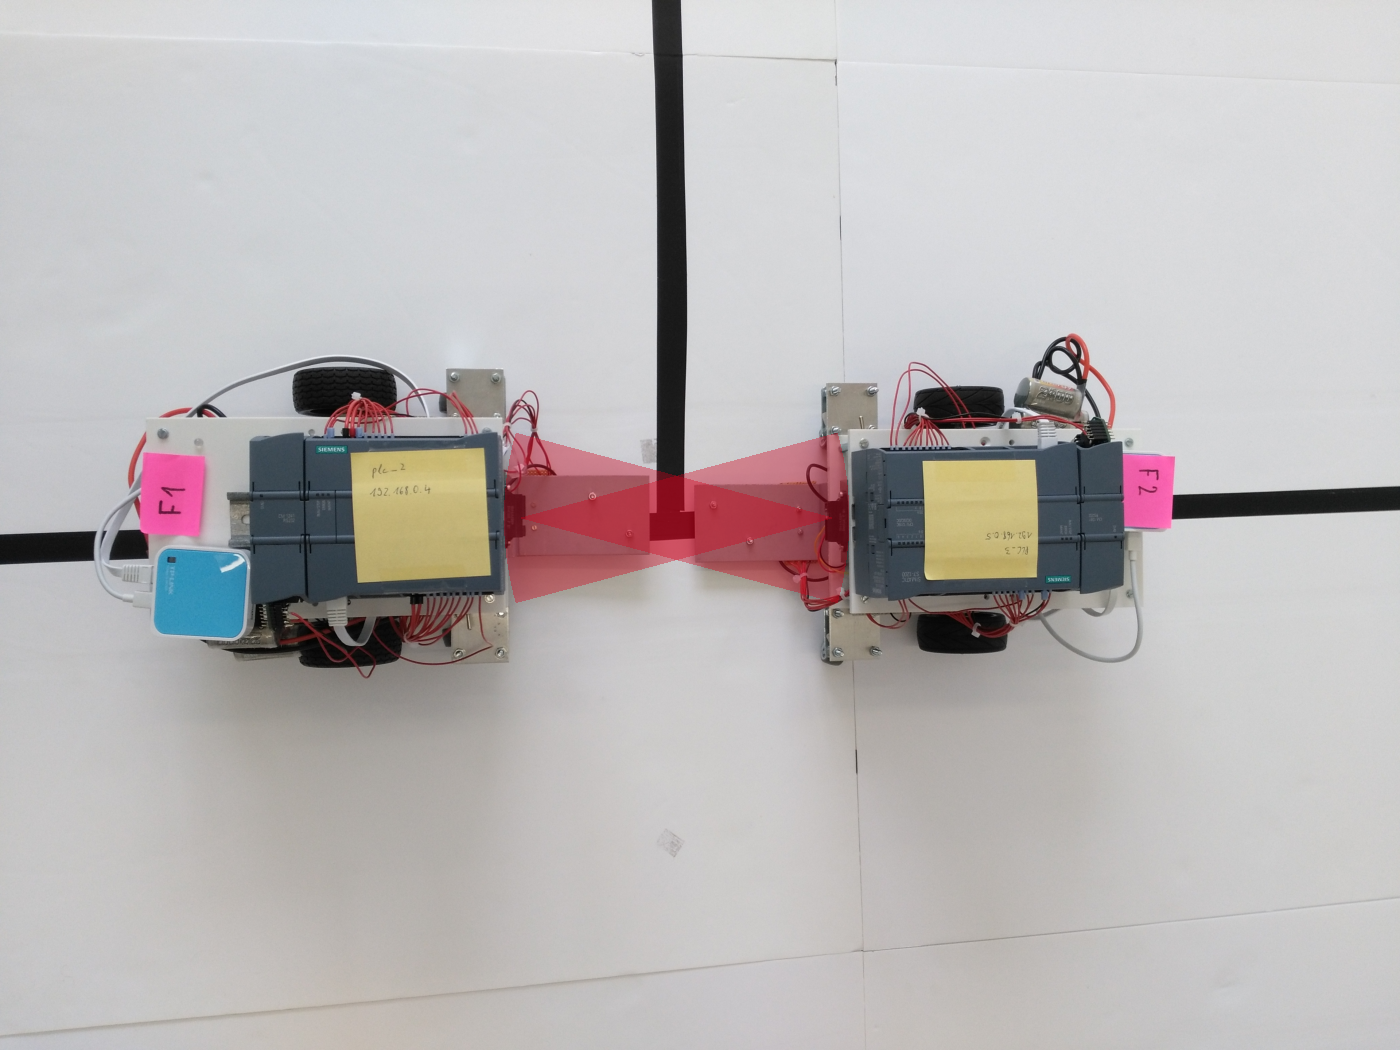
\includegraphics[scale=0.7, trim = 15mm 50mm 25mm 50mm, clip]{/Bilder/FrontalKollisionPDF}
			\vspace{0.2cm}
			\caption{Deadlock bei zu lang eingestellten Kollisionssensoren. Fahrzeuge erkennen sich gegenseitig bevor sie die Kreuzung erreichen.}\label{FronalKollision}
		\end{figure}
		
		Zur Lösung dieses Problems muss entweder den Fahrzeugen eine Priorität beim Einfahren am selben Knoten vergeben werden, damit das niedrigpriore \ac{FTF} die Kreuzung für das hochpriore Fahrzeug freigibt, oder eine solche Annäherung an den gleichen Zielknoten muss algorithmisch verhindert werden. Da im Normalfall eine Reaktion auf andere Fahrzeuge jedoch funktioniert und zum Projektende die Zeit für eine Implementierung und nachfolgende Tests dieser zusätzlichen Funktionen nicht zur Verfügung stand, wurde eine Lösung für dieses Problem bisher noch nicht implementiert.
		\\[4pt]
		Ähnlich zu der soeben beschriebenen Situation kann es passieren, dass zwei Fahrzeuge kollidieren, wenn sie sich zeitnah seitlich im 90°-Winkel an eine Kreuzung annähern. Da die Kollisionssensoren nur Hindernisse vor sich erkennen können, kann es vorkommen, dass sich die Sensorausleger verkeilen, wenn die Fahrzeuge ungefähr zeitgleich in die Kreuzung einfahren. Abbildung \ref{SideKollision} zeigt, wie sich die Fahrzeuge aufgrund der Sensoranordnung gegenseitig nicht erkennen und gleichzeitig versuchen in die Kreuzung einzufahren. Zum Abfangen dieser Situation bedarf es jedoch zusätzlicher Sensoren seitlich am Fahrzeug, die an Kreuzungen quer fahrende Fahrzeuge detektieren können. Ein Umbau der Hardware des \ac{FTF} war jedoch zeitlich nicht mehr realisierbar.
		
		\begin{figure}[h]
			\centering
			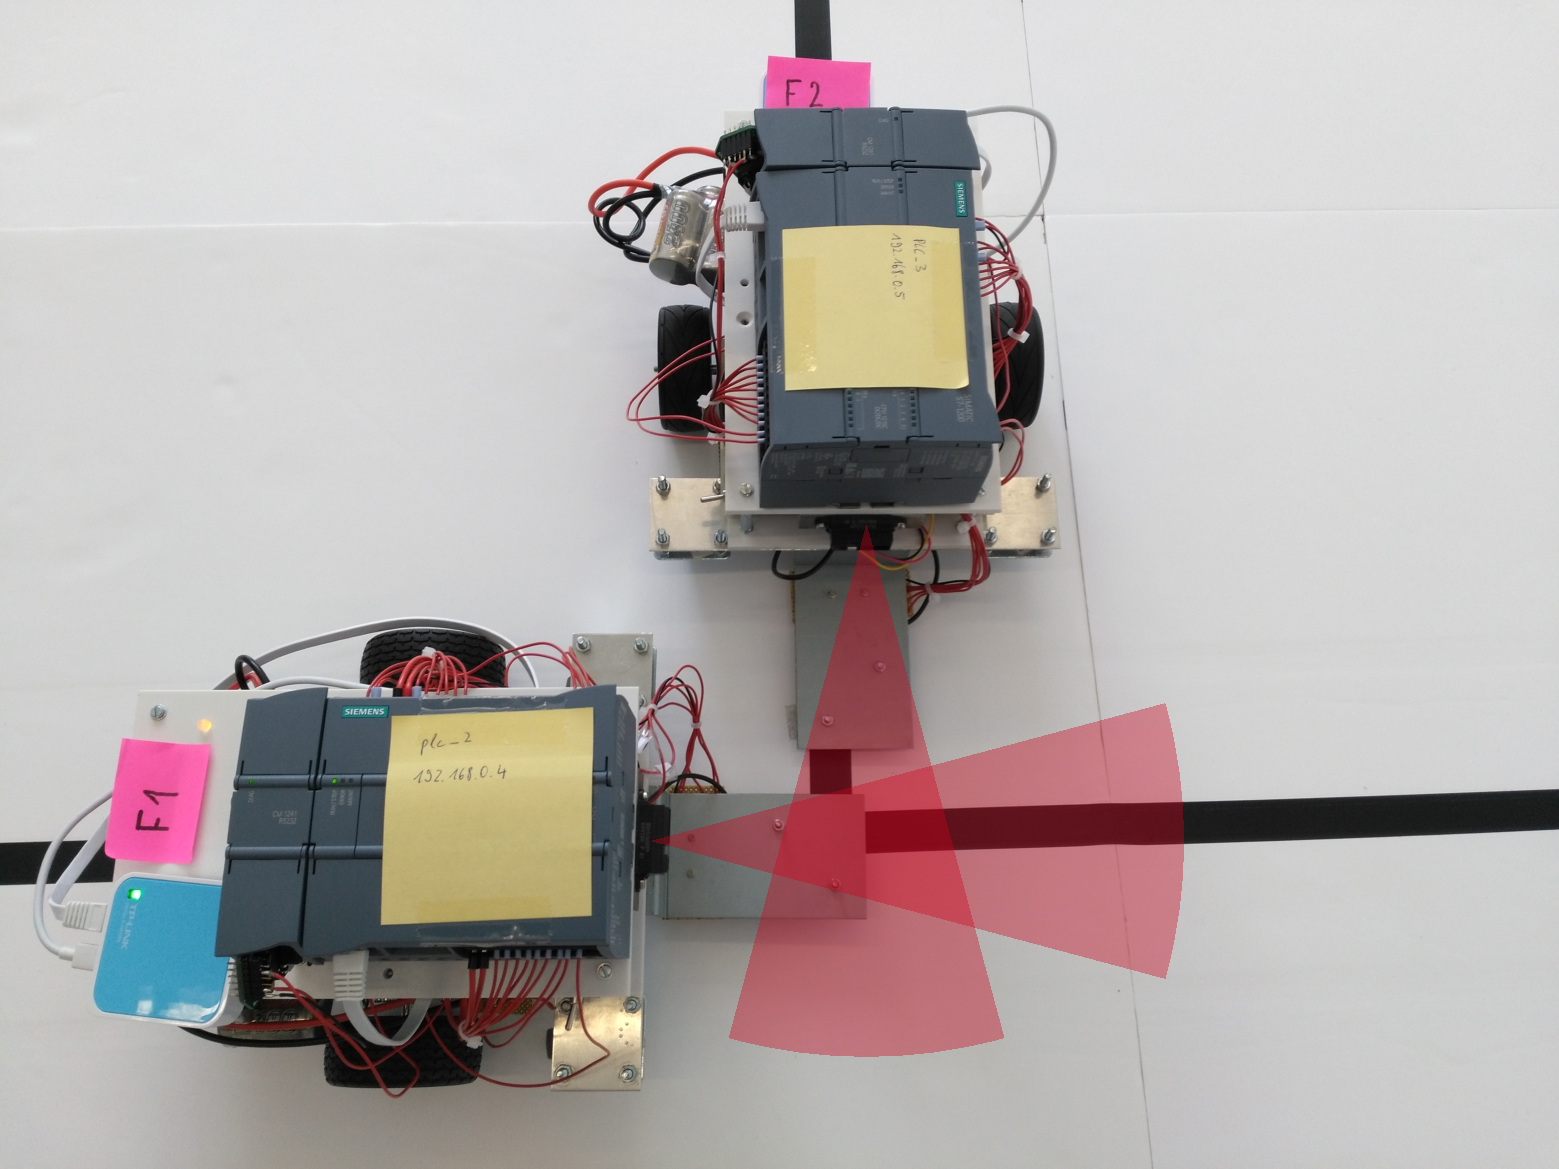
\includegraphics[scale=0.6, trim = 5mm 5mm 55mm 5mm, clip]{/Bilder/SideKollisionPDF}
			\vspace{0.2cm}
			\caption{Situation bei bevorstehender, seitlicher Kollision an einer Kreuzung. Kreuzende Fahrzeuge werden nicht durch den Frontalsensor erkannt.}\label{SideKollision}
		\end{figure}
	
\section{Ausblick über zukünftige Erweiterungen}
	
	Als wichtigster nächster Schritt ist zunächst die Implementierung der in Abschnitt \ref{Probleme_Hardware} beschriebenen Lösungen zur Verhinderung von Kollisionen an Kreuzungen zu erwähnen. Dies verhindert die vereinzelt auftretenden fatalen Fehler, die einen manuellen Eingriff erfordern.\\
	Eine weitere  geplante Anlagenerweiterung ist die Auslagerung der in Abschnitt \ref{Simulation Station} beschriebenen Simulation der Bearbeitungszeit an die jeweiligen Steuerungen der Stationen. Geplant ist hier ein Anmelden des Fahrzeugs an der jeweiligen Bearbeitungsstation und eine Rückmeldung der Station, sobald die Bearbeitung abgeschlossen ist. Dies ermöglicht unterschiedliche Bearbeitungszeiten an unterschiedlichen Maschinen und lässt somit eine bessere Analyse des Werkstückflusses durch die Anlage zu. Es könnte hier zum Beispiel untersucht werden, inwiefern die doppelte Ausführung von Stationen mit langer Bearbeitungszeit einen Einfluss auf die Produktivität der Anlage haben.
	\\[4pt]
	Ähnlich der Auslagerung der Bearbeitungszeit ist auch eine zentrale Zuweisung von Rezepten beim Einfahren in die Anlage in Planung. Dies simuliert die Anbindung an ein der Anlage übergeordnetes Betriebsleitsystem\footnote{englisch: \ac{MES}}, welches zentral bestimmt, welche Art von Produkten benötigt wird und dann bei Bedarf das passende Rezept an einen Werkstückträger in der Anlage zuweist.
	\\[4pt]
	Zudem ist geplant, die Bearbeitungsschritte innerhalb eines Rezeptes variabler zu gestalten. So soll es beispielsweise möglich sein, dass es für ein Werkstück egal ist, in welcher Reihenfolge die  Bearbeitungsschritte 3, 4 oder 5 abgearbeitet werden. Einzige Voraussetzung soll sein, dass alle Schritte ausgeführt wurden bevor Bearbeitungsschritt 6 ausgeführt wird. Dies ermöglicht eine erhöhte Dynamik innerhalb der Anlage, da es in diesem Fall möglich ist, zunächst die Bearbeitungsstation für die Funktionalität 5 als Ziel auszuwählen, wenn zu diesem Zeitpunkt alle Bearbeitungsstationen mit der Funktion 4 bereits belegt sind.
	\\[4pt]
	Eine letzte gewünschte Zusatzanforderung ist die Weiterentwicklung der Visualisierung der Anlage. Diese soll so erweitert werden, dass auf dem Bildschirm ein einzelnes aktives Fahrzeug ausgewählt und teilweise gesteuert werden kann. Somit soll beispielsweise eine Manipulation der Reihenfolge von Bearbeitungsschritten des aktuellen Rezeptes möglich sein, oder die Zuweisung eines komplett neuen Rezeptes. Dies würde ein gewisses Maß an Interaktion bei Vorführungen der Modellanlage bei Kunden ermöglichen.

\section{Zusammenarbeit mit der Entwicklungsabteilung \ac{CT}}

	Parallel zur Entwicklung der Anlage wurde mit der Entwicklungsabteilung der Siemens AG die Grundlage für eine Simulation der realisierten Anlage gelegt. Der Anlagenaufbau sowie Teile der Funktionalität wurden gemeinsam definiert und Use-cases formuliert, die innerhalb einer rechnergestützten Simulation der Anlage mit den Daten des realen Modells verglichen werden können. Zudem kann in bestimmten Zeitintervallen der Zustand der Simulation mit dem wirklichen Anlagenzustand synchronisiert werden. Dies würde es theoretisch ermöglichen, die in Abschnitt \ref{Zeitproblem} erwähnte einstufige Routenvorhersage zu verbessern. Da der Simulation zusätzliche Informationen über alle Fahrzeuge zur Verfügung stehen, welche die Wegfindung aufgrund ihres dezentralen Aufbaus nicht nutzen kann, wäre es denkbar, dass durch Rückmeldung der Simulation an die einzelnen Steuerungen die Wegfindung verbessert werden kann, ohne diese bei Ausfall des zentralen Rechners komplett zu verlieren.
	
\section{Bewertung des Projekts}
	
	Vor Beginn des Projekts war ich zunächst etwas skeptisch, dass sich eine derartig komplexe Funktion wie die Wegfindung auf einem System mit so vielen Beschränkungen wie eine \ac{SPS} überhaupt realisieren lassen würde. Bei der Recherche wurde aber schnell klar, das es grundsätzlich nicht nötig ist, die Wegfindung auf ein PC-System auszulagern, sondern das diese Aufgabe komplett auf einer industriellen Steuerung realisierbar ist. Vor allem die Überwindung von Stolpersteinen bei der Implementierung brachte interessante Herausforderungen, die zu Beginn des Projektes noch gar nicht absehbar waren. Es ist jedoch auch zu sagen, dass die Realisierung einer derartigen Funktion etwas zeitaufwendiger ist als eine vergleichbare Lösung auf einem PC, da auf der PC-Seite oft auf bestehenden Lösungen aufgebaut werden kann. Dies ist bei der Implementierung auf einer \ac{SPS} nicht der Fall. Trotz des Fehlens eines Debuggers und dem damit verbundenen erhöhten Entwurfsaufwands war vor allem die Herausforderung der Aufgabe ein Ansporn, nicht nur ein funktionierendes, sondern auch ein effizientes Wegfindungssystem zu entwickeln. Durch die übergeordnete Aufgabe des Entwurfs einer Modellanlage und die dadurch greifbaren Ergebnisse war das Projekt auch für mich, als eher an der Programmierung interessiertem Menschen, eine interessante Aufgabe. Durch die Zusammenarbeit mit dem Bearbeiter der Fahrzeugsteuerung wurde auch das Arbeiten innerhalb eines Teams mit Eigenverantwortung für die eigenen Themenbereiche gut erprobt und bewältigt.

\section{Zusammenfassung}
	
	Viele Aspekte von Industrie 4.0 werden in den kommenden Jahren immer mehr an Bedeutung gewinnen. Aus diesem Grund ist es für Firmen unabdingbar, ihre Produktion so effizient wie möglich zu gestalten. Im Zuge dessen halten vermehrt Konzepte der IT und der klassischen Informatik Einzug in den Produktionsablauf. Unter diesem Gesichtspunkt ist es interessant zu untersuchen, inwiefern sich diese Konzepte in die Abläufe der Automatisierungstechnik einbinden lassen. Diese Arbeit zeigt, dass es generell möglich ist, selbst komplexere Algorithmen auf industriellen Standardsteuerungen zu realisieren. Durch die Implementierung eines dezentralen Wegfindungsalgorithmus auf Basis des A*-Algorithmus mit exakter Heuristik, wurde auf einer \ac{SPS} der S7-1200er Reihe eine beispielhafte Implementierung erarbeitet. Trotz der Beschränkungen der Steuerungen bezüglich des Speicherplatzes und der Vorhersagbarkeit der Bewegungen anderer Fahrzeuge, lässt sich mittels geeigneter Handhabung der Fahrzeuginformationen verhindern, dass sich die Fahrzeuge in den meisten Fällen gegenseitig behindern. Ganz lässt sich die Wahrscheinlichkeit einer Kollision zum derzeitigen Stand der Anlage noch nicht vermeiden, jedoch wurde der Weg für eine Behebung dieser und anderer Schwachstellen aufgezeigt. Die Routenberechnung ermöglicht es in Verbindung mit dem implementierten Fahrerlosen Transportsystem, Werkstücke anhand verschiedener Rezepturen innerhalb der gleichen Produktionslinie gemeinsam produzieren zu können. Anhand der realisierten Modellanlage lassen sich somit die Industrie4.0-Konzepte der Dezentralisierung, des autonomen Fahrens sowie der Anlagenskalierbarkeit in geeigneter Form darstellen und für potentielle Kunden vorführen.
	
	